\ifpdf
	\graphicspath{{2/pic/PNG/}{2/pic/PDF/}{2/pic/}}
\else
	\graphicspath{{2/pic/EPS/}{2/pic/}}
\fi

\chapter{Mathematical model of neutron transport}\label{chap:nte-review}

\nomenclature[s]{$f \approx g$}{$f$ is approximated by $g$}
\nomenclature[s]{$f \equiv g$}{$f$ is by definition equivalent to $g$}
\nomenclature[a]{$\R[n]$}{an n-dimensional Euclidean vector space}

The steady state neutron transport equation is a mathematical representation of balance between neutron gains and losses
within a given macroscopic domain $\VV\subset\R[3]$. Let us consider the equation in its integro-differential form with
given neutron source function $Q$:
\begin{equation}\label{eq0}
  \begin{multlined}
    \Bigl[
      \bomega\cdot\grad + \sigma_t(\br,\bomega,E)
    \Bigr]
    \psi(\br,\bomega,E) =\\
    = \intE[']{\Emin}{\Emax}{\intA[']{\kappa(\br,\bomega\sla\bomega',E\sla E')\psi(\br,\bomega',E',t)}}  + 
    \src(\br,\bomega,E).
  \end{multlined}  
\end{equation}
Function $\sigma_t$ groups all reactions that result in a loss of neutron, while $\kappa$ represents reactions that
introduce neutrons into direction $\bomega$ and energy $E$ by, e.g., scattering from direction $\bomega'$, slowing down
from energies $E'$ or release from fissioned nuclei.
They are given by material composition of the domain and we will return to their more detailed description, as
well as to boundary conditions when $\VV$ is bounded, in section \ref{sec:NTE}.

Solution of eq. \eqref{eq0}, the \textit{angular neutron flux density} $\psi$ -- is a function of the following
independent variables, which define the neutron phase space:
\begin{itemize}
 	\item $\br = (x,y,z)$
 	\nomenclature[A]{\br}{position vector}
 	\nomenclature[U]{x,y,z}{components of vectors in Cartesian coordinate system} represents the spatial distribution of
 	 neutrons,
 	\item $\bomega$\nomenclature[g]{$\bomega$}{unit vector of neutrons flow direction} represents the angular
 	distribution of neutrons on a unit sphere $\Sphere$\nomenclature[A]{\Sphere}{unit sphere ($\{x\in\R[3]: \norm{x} =
 	1\}$)} ,i.e. their flow direction ($\br\in\R[3]$, $\norm{\br}=1$);
 	\item $E\in [E_{\text{min}},E_{\text{max}}]$\nomenclature[g]{$E$}{Energy of neutrons\nomunit{eV}} is the kinetic
 	energy of neutrons
\end{itemize}

\begin{remark}
	The phase space could be also defined in terms of the velocity vector $\bv$ and speed $v = \norm{\bv} = \sqrt{2E/m}$
	($m$ being the mass of neutron) instead of $\bomega$ and $E$. 
	This form appears to be preferred in analytical works, while our choice is more often used in practical numerical
	calculations.
	Corresponding changes in the formulation of the NTE are
	explicitely given e.g. in \cite[Chap. XXI, eqns. (1.1) and (1.2)]{DautrayLions}. For further use, we will just note
	that we can write $\bomega = \bv / v$ with $\bv\in\R[3]$.
\end{remark} 
\begin{remark}
	In this macroscopic description, we should always consider beams of neutrons with the same given average properties in
	differential elements around $\br$, $\bomega$, $E$. For simplicity, we will refer to them as to single neutrons with
	particular position, energy or direction (and occassionally call them $(\br,\bomega,E)$-neutrons) and we also omit the
	``density'' specification of repeatedly used quantities -- e.g., we will henceforth call $\psi$ just \textit{angular neutron flux}.
\end{remark} 

\section{Neutron phase space} \label{sec:phase}
Let us assume that $\VV$ is a domain bounded by a piecewise smooth boundary $\pV$, which may be oriented at almost every
point $\br\in\pV$ (a.e. in $\pV$) by its unit outward normal field $\bn(\br)$. 
Then we may formally define the neutron phase space 
$$
  X := \{(\br,\bomega,E):\ \br\in \VV\subset\R[3], \bomega\in \Sphere, E \in [\Emin,\Emax]\}
$$
together with its outflow and inflow boundary subsets, respectively:
$$
  \pX[\pm] := \bigl\{ (\br,\bomega,E) \in \pV \times \Sphere \times [E_m, E_M], \mbox{ s.t. } \bomega\cdot\bn(\br)
  \gtrless 0 \bigr\}
$$%
\begin{figure}[!hbt]
    \centering
    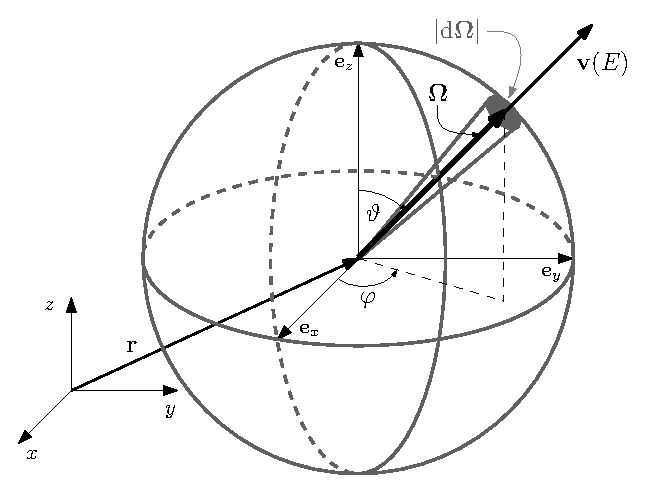
\includegraphics[scale=1]{phase_space.eps}
    \caption[Phase space of neutrons]{Phase space of neutrons}
    \label{fig:phase_space}
\end{figure}%
The product measure
\begin{equation}\label{eq:measure}
  \d{x} = \d{\mu(X)} = \d{\mu(V\times\Sphere\times [\Emin,\Emax])} = \d{\br}\d{\bomega}\d{E}
\end{equation}
is used when integrating over $X$, 
while the boundary measure
\begin{equation}\label{eq:measure2}
\db = \abs{\bomega\cdot\bn}\d{\gamma}\d{\bomega}\d{E},\quad \d{\gamma} = \d{\mu(\pV)},
\end{equation}
is used when integrating over $\pX[\pm]$. When refering to physical units, we will consider the length scale of $\VV$ in
centimeters.

Since the direction vectors are confined to the sphere, we can express the three
Cartesian components of $\bomega$ by only two spherical coordinates $\polar\in[0,\pi]$ and
$\azimuthal\in[0,2\pi)$\nomenclature[g]{$\polar$}{polar angle}\nomenclature[g]{$\azimuthal$}{azimuthal
angle}:
\begin{equation*}
	\bomega = \left[\begin{array}{c}
		\Omega_x \\
		\Omega_y \\
		\Omega_z
	\end{array}\right] = \left[\begin{array}{c}
		\sint\cosp \\
		\sint\sinp \\
		\cost
	\end{array}\right]
\end{equation*}
(see \fref{fig:streaming}).
\begin{figure}[!hbt]
    \centering
    \includegraphics[scale=1.125]{cartesian_streaming}
    \caption[Cartesian coordinate system]{Cartesian coordinate system}
    \label{fig:streaming}
\end{figure}
To transform integrals with respect to $\d{\bomega}$ into double integrals with respect to $\polar$ and $\azimuthal$,
note that the solid angle $\d{\bomega}$ subtended at the center of $\Sphere$ by the spherical differential element
$\abs{\d{\bomega}}$ can be written as:
$$
	\d{\bomega} = \frac{\abs{\d{\bomega}}}{r^2} = \frac{r^2 \sint \d{\polar}\d{\azimuthal}}{r^2} =  \sint
	\d{\polar}\d{\azimuthal} $$
(see \fref{fig:element}).
\begin{figure}[!hbt]
    \centering
    \includegraphics[scale=1.275]{element}
    \caption[Solid angle]{Schematic of the (scaled) solid angle of directions}
    \label{fig:element}
\end{figure}

\section{Steady state neutron transport in isotropic bounded domain}\label{sec:NTE}
In most practical cases, we can assume that the medium in which we study neutron transport is isotropic.
The first consequence of this assumption is that 
$$
	\sigma_t(\br,\bomega,E)\psi(\br,\bomega,E) \equiv \sigma_t(\br,E)\psi(\br,\bomega,E)
$$ 
for any $\bomega\in\Sphere$. The
second is that reactions that change the direction of neutrons from $\bomega'$ to $\bomega$ are
invariant under rotation of the coordinate system and are thus completely determined by the cosine of the two vectors:
$$
	\kappa(\cdot,\bomega\sla\bomega',\cdot) \equiv \kappa(\cdot,\bomega\cdot\bomega',\cdot).
$$
The steady state NTE \eqref{eq0} in this regime reads
\begin{equation}\label{eq1}
\begin{multlined}
  \bomega\cdot\nabla\psi(\br,\bomega,E) + \sigma_t(\br,E)\psi(\br,\bomega,E) =\\[.25em]
   = \intE[']{\Emin}{\Emax}{
      \intA[']{\kappa(\br,\bomega\cdot\bomega',E\sla E')\psi(\br,\bomega',E')}
    } + q(\br,\bomega,E)
 \end{multlined}
\end{equation}
in $X$, complemented by specified angular flux distribution at $\pX[-]$. The two prototypical inflow boundary
conditions are:
\begin{itemize}
	\item incoming angular neutron flux
	\begin{equation}\label{eq:nte2}
	  \psi\vert_{\pX[-]} = \psi_{\text{in}}
	\end{equation}
	($\psi_{\text{in}}\equiv 0$ corresponds to vacuum in $\R[3]\setminus \overline V$, which is a common
	 assumption in nuclear reactor modeling),
	
	\item albedo boundary reflection
	\begin{equation}\label{eq:nte3}
  	\psi(\br,\bomega,E) = \alpha(\br)\psi(\br, \bomega_R, E),\quad (\br,\bomega,E)\in \pX[-],\ \ \bomega_R = \bomega - 2
  	\bn (\bomega \cdot \bn)
  \end{equation}
  where $\bomega$ is the reflection of $\bomega_R$ about the boundary plane. For $\alpha \equiv 1$, this corresponds to
  complete specular reflection and is used to model planes of symmetry, while for $\alpha =
  0$, we recover the vacuum condition from above. Intermediate values mean that a fraction of neutrons leaving the
  domain in direction $\bomega_R$ are returned back in direction $\bomega$, which is commonly used to model reactor
  reflectors. We thus assume $0 \leq \alpha \leq 1$. 
\end{itemize}
\begin{remark}
	The albedo coefficient $\alpha$ may in general vary with the reflector properties and should also capture 
	redistribution of the reflected neutrons within the phase space due to their diffusion through the reflector. A general
	treatment of albedo condition is given in \cite{Sanchez4} (see also \cite{Sanchez3}), where an integral albedo operator
	$\beta$ is introduced, such that
\begin{equation}\label{eq:albedo-general}
	\angflux(x)\big\vert_{\pX[-]} = (\beta\angflux)(x) = \bndint[']{\pX[+]}\beta(x'\sra x)\angflux(x'),
\end{equation}
	where $x = (\br,\bomega,E)$ and $x' = (\br',\bomega',E')$. 
\end{remark}
For formal description of other types of boundary conditions, we refer to \cite{Sanchez4} or \cite[Sec. 1.3]{Agoshkov}.

A physically plausible solution of NTE should be moreover non-negative throughout $\VV$ and continuous along any
direction $\bomega$, i.e. $\psi(\br + s\bomega,\bomega,E)$ is a continuous function of $s$ for any $\br$, $\bomega$, $E$. Note
that $\psi(\br + s\bomega',\bomega,E)$ \textsl{may} be discontinuous when $\bomega' \neq \bomega$.

\subsection{Advection term}\label{sec:advection}
In Cartesian coordinate system (that we will exclusively consider in this thesis),
$$
	\bomega\cdot\nabla\angflux = \bomega_x\pd{\angflux}{x} + \bomega_y\pd{\angflux}{y} + \bomega_z\pd{\angflux}{z} = 
	\der{x}{s}\pd{\angflux}{x} + \der{y}{s}\pd{\angflux}{y} + \der{z}{s}\pd{\angflux}{z} = \der{\angflux}{s},
$$
where $s\in I\subset \R$ parametrizes the path traveled by the neutron along the direction $\bomega$ (the
\textit{characteristic}, see \fref{fig:cartesian2}).
\begin{figure}[htp]
\begin{center}
  \includegraphics[scale=1.2]{cartesian_streaming2}
  \caption{Characteristic direction in the Cartesian coordinate system}
  \label{fig:cartesian2}
\end{center}
\end{figure}
Assuming now for simplicity that the integral term on the right of \eqref{eq1} is absorbed in the source term $q$, we
may invert the differential operator on the left of \eqref{eq1} by integration along these characteristics and obtain an
integral formulation of the neutron transport equation:
\begin{equation}\label{eq:nte-integral}
	\angflux(\br,\bomega) = \angflux(\br_0,\bomega)e^{-\tau(\br,\br_0)} + \int_0^{s_0}
	q(\br',\bomega)e^{-\tau(\br,\br')}\,\d{s'}
\end{equation}
where
\begin{align}
	\br' &= \br - s' \bomega, \quad \br_0 = \br - s_0 \bomega\nonumber\\[.2em]
	\tau(\br,\br') &= \tau(\br,\br-s'\bomega) = \int_0^{s'} \Sigma_t(\br - s''\bomega)\,\d{s''} \label{eq:tau}
\end{align}
In reference to \fref{fig:trepka}
\begin{figure}[hbp]
\begin{center}
  \includegraphics[scale=.75]{trepka}
  \caption{Illustration for the solution on a characteristic}
  \label{fig:trepka}
\end{center}
\end{figure}
we can interpret the first term on the right of \eqref{eq:nte-integral} as the number of
neutrons moving in the direction $\bomega$ that entered the given volume in $\br_0$ and reached point $\br$ without
collision, whereas the second term as the number of neutrons introduced into the characteristic direction by sources 
between $\br_0$ and $\br$ and reaching $\br$ without collision. The \textit{optical path length} $\tau$ represents the 
probability of collision between $r'$ and $r$. This integral form is of both theoretical and practical value, as we will
see later in sections \ref{sec:fixed-source} and \ref{sec:lattice}.

\subsection{Collision terms}
The kernel of the integral operator on the right-hand side of \eqref{eq1} can be split into the so-called
\textit{double-differential macroscopic cross-section} for scattering and fission, respectively:
\begin{equation}\label{eq:splitting}
  \kappa(\br,\bomega\cdot\bomega',E\sla E') = \sigma_s(\br,\bomega\cdot\bomega',E\sla E') +
  \sigma_f(\br,\bomega\cdot\bomega',E\sla E').
\end{equation}
These cross-sections characterize the mean number of ($\bomega$, $E$)-neutrons coming out of a (possible) collision of 
($\bomega'$, $E'$)-neutrons with nuclei at $\br$ (or more precisely in a
differential element around $\br$). Note that the collision can either just change the direction and energy of the
inducing neutrons (inelastic scattering) or cause absorption of the neutrons followed by release of
new ones in the considered direction and energy range (fission), or both (elastic scattering\footnote{As inelastic
scattering is dominant in our applications, we will not treat elastic and inelastic scattering separately and include 
both types in $\sigma_s(\br,\bomega\cdot\bomega',E\sla E')$}).
Ordinary macroscopic cross-sections $\sigma_s(\br,E)$, $\sigma_f(\br,E)$ are then introduced to characterize the
probability that neutrons undergo collisions of the above type irrespective of the outcome, i.e.
\begin{equation}\label{eq:ddifxs}
\begin{aligned}
\eta\sigma_s(\br, E) &= \intE[']{\Emin}{\Emax}{\intAA{\sigma_s(\br,\bomega\cdot\bomega', 
	E\shortrightarrow E')}},\\
\nu\sigma_f(\br, E) &= \intE[']{\Emin}{\Emax}{\intAA{\sigma_f(\br,\bomega\cdot\bomega', 
	E\shortrightarrow E')}}
\end{aligned}
\end{equation}
where $\eta$ and $\nu$, respectively, are the mean number of neutrons coming out of the scattering event ($=1$ in case
of purely inelastic scattering, $> 1$ for elastic scattering) and the fission event, respectively.

The \textit{total macroscopic cross-section}, $\sigma_t$, characterizing the probability that neutron with energy $E$
undergoes a collision of any type with nuclei at $\br$, can now be decomposed as 
\begin{equation}\label{eq:st}
  \sigma_t(\br,E) = \sigma_c(\br,E) + \sigma_f(\br,E) + \sigma_s(\br,E) \equiv \sigma_a(\br,E) + \sigma_s(\br,E)
\end{equation}
where
\begin{itemize}
	\item $\sigma_c(\br, E)$ is the non-productive capture cross section (resulting in no new neutrons being introduced
	into the system) and
  	\item $\sigma_a(\br, E) = \sigma_c(\br,E) + \sigma_f(\br,E)$ is the absorption cross section.
\end{itemize}

For later use, note that fission is an isotropic process (which removes the angular dependence of the
double-differential fission cross-section altogether) and the new energy distribution does not depend on the energy of 
the inducing neutron 
\begin{figure}[hbt]
\begin{center}
  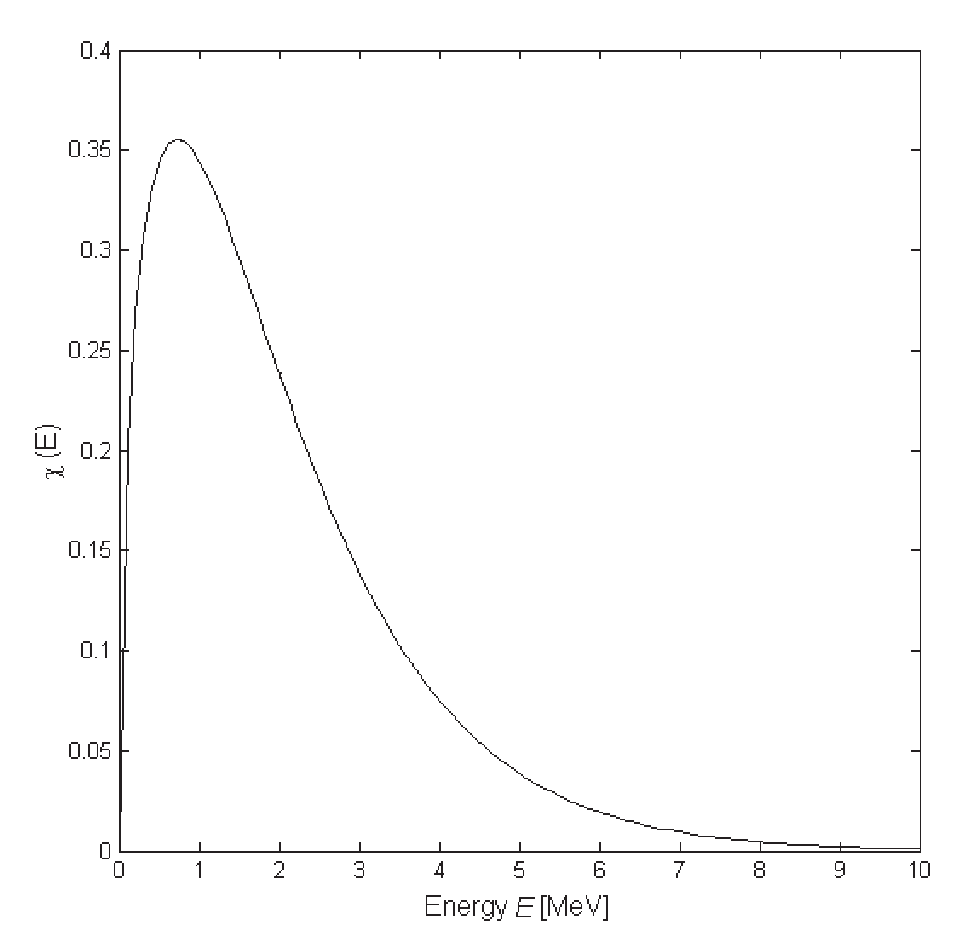
\includegraphics[scale=.6]{spectrum}
  \caption{Energy spectrum of neutrons released from fission of U235}
  \label{fig:spectrum}
\end{center}
\end{figure}
(as it corresponds to the neutrons originally bound inside the nucleus; \fref{fig:spectrum}
shows a typical shape of that function); using the second eq.
\eqref{eq:ddifxs}, we can then write:
\begin{equation}\label{eq:sf}
\sigma_f(\br,\bomega\cdot\bomega',E\sla E') = \frac{\chi(E)\nu\sigma_f(\br,E')}{4\pi},\quad 
\intE[']{\Emin}{\Emax}{\chi(E')} = 1
\end{equation}

A physically realistic assumption is that all the macroscopic cross-sections are bounded measurable functions
 \footnote{with respect to product measure of type \eqref{eq:measure} appropriate for their particular set of arguments,
 or with respect to $\d{\mu(V\times\Sphere^2\times [\Emin,\Emax]^2)}$ in case of double-differential cross-section},
 piecewise continuous in $\VV$. The unit of macroscopic cross-sections is \SI{}{cm^{-1}}.

\subsection{Quantities of importance}
From the solution of eq. \eqref{eq:bte1}, one can derive the following integral quantities
\begin{itemize}
  \item \textit{scalar neutron flux density} \SI{}{[cm^{-2}.s^{-1}]}
  \begin{equation*}%\label{eq:scalar_flux}
    \phi(\br, E) = \intA{\psi(\br,\bomega,E)},
  \end{equation*}
  \item \textit{net neutron current density} \SI{}{[cm^{-2}.s^{-1}]}
	\begin{equation*}%\label{eq:bJ}
		\bJ(\br, E)	= \intA{\bomega\psi(\br,\bomega,E)},
	\end{equation*}
\end{itemize}
so that integrating $\bJ(\br,E)\cdot\bn(\br)$ over a given surface 
gives the total number of neutrons with energy $E$ crossing (per unit time) that surface in the direction of 
$\bn$. Also,
\begin{equation}\label{eq:rr}
  \intE{E_1}{E_2}{\sigma_x(\br, E) \phi(\br, E)}
\end{equation}
represents the \textit{reaction rate density} (per unit time) of given type ($x = t,a,f,s,c$, see \eqref{eq:st}), 
induced by neutrons of energies in range $[E_1, E_2]$. 
These quantities produce directly observable effects and may be experimentally measured
by various detector mechanisms, which is the reason why they are more important in practical calculations than the 
actual solution of the NTE (i.e. the angular neutron flux). Note that for the total volumetric scalar flux to be finite 
(as is physically expected), we should look for the solution $\psi$ of the NTE in the space $\Lp[1](X)$ with boundary 
values in $\Lp[1](\pX[\pm])$ (equipped with the respective measures defined in Sec. \ref{sec:phase}), which is 
therefore usually taken as the natural function space setting (\cite{DautrayLions}).
Of particular importance for reactor calculations is the
\begin{itemize}
  \item \textit{power density} \SI{}{[W.cm^{-3}]}
\begin{equation}\label{eq:power}
	\intE{\Emin}{\Emax}{e\sigma_f(\br, E) \phi(\br, E)}
\end{equation}
	where $e$ is the energy conversion factor converting fission rate to watts.
\end{itemize}

In the following, we will formulate the two basic problems of neutron transport in an operator form.
We will consider the generalized statements in which the equation and boundary conditions are assumed to be satisfied a.e. in $X$ and
$\bomega\cdot\nabla$ represents the generalized derivative in the usual Sobolev sense. This is motivated by the low
regularity that can be expected from the exact solution of the NTE -- for example, even for piecewise smooth material data
(cross-sections $\sigma_x$) and sources $q$, the solution of the NTE is known to possibly exhibit singularities in 
first partial derivatives (or be discontinuous as a function of $\bomega$) at surfaces of material discontinuities 
coinciding with characteristic curves of the left-hand side of \eqref{eq1} (\cite[Chap. 1]{Agoshkov}, \cite[Sec.
III]{Vladimirov}).

\subsection{Neutron transport problem with fixed sources}\label{sec:fixed-source}
Let us introduce the standard spaces of Lebesgue-integrable functions (w.r.t. the product measure \eqref{eq:measure},
resp. \eqref{eq:measure2}) $$
\nomenclature[a]{$\Lp(X)$}{space of functions integrable in the Lebesgue sense with their $p$-th power over $X$}
\nomenclature[a]{$\Lp_\sigma(X)$}{space weighted with the total cross-section $\sigma_t$}
\begin{aligned}
	\Lp(X) &= \left\{\psi\mid \norm[\Lp(X)]{\psi} := \left(\int_X\abs{\psi(x)}^p\,\d{x}\right)^{1/p} <
	\infty\right\},\quad 1\leq p < \infty,\\
	\Lp(\pX[\pm]) &= \left\{\psi\mid \Vert\psi\Vert_{\Lp(\pX[\pm])} :=
	\left(\int_{\pX[\pm]}\abs{\psi(x)}^p\,\db\right)^{1/p} < \infty\right\},\quad 1\leq p < \infty,\\
	\Lp[\infty](X) &= \{\psi\mid \norm[L^{\infty}(X)]{\psi} := \esssup_{X} \abs{\psi(x)} < \infty\}\\
	\Lp[\infty](\pX[\pm]) &= \{\psi\mid \Vert\psi\Vert_{L^{\infty}(\pX[\pm])} := \esssup_{\pX[\pm]}
	\abs{(\bomega\cdot\bn)\psi(x)}< \infty\}
\end{aligned}
$$
and let
$$
  \nomenclature[a]{$\Hp{p}(X)$}{Sobolev space of functions whose (generalized) partial derivatives up to order $k$ are
 in $\Lp{p}$.} 
 \Hp(X) = \left\{\psi\in\Lp(X), \bomega\cdot\nabla\psi\in\Lp(X)\right\} 
$$
We formulate the fixed source problem using the following operators:
\begin{equation*}
  \begin{gathered}
    A\psi(\br,\bomega,E) = \bomega\cdot\nabla\psi(\br,\bomega,E),\\%[.85em]
    \Sigma_t\psi(\br,\bomega,E) = \sigma_t(\br,E)\psi(\br,\bomega,E),\\%[.75em]
    K\psi(\br,\bomega,E) = \intE[']{\Emin}{\Emax}{
            \intA[']{\kappa(\br,\bomega\cdot\bomega',E\sla E')\psi(\br,\bomega',E')}
          }.
  \end{gathered}
\end{equation*}
We shall call $A$, $\Sigma_t$, $K$ and $T = A + \Sigma_t - K$ the \textit{advection}, \textit{collision}, 
\textit{transfer} and \textit{transport} operator, respectively. The collision operator $\Sigma_t : \Lp(X) \to
\Lp(X)$ is self-adjoint and bounded, while the operator $K: \Lp(X) \to \Lp(X)$ is bounded under additional
(physically justifiable) conditions (conditions (c) and/or (d) of the following theorem, depending on the chosen $p$) as
a consequence of H\"older inequality (\cite[Chap. XXI, \S 2]{DautrayLions}), but is self-adjoint if and only if
the kernel $\kappa$ of $K$ is symmetric in $E$ and $E'$. With the exception of the mono-energetic case, this is
generally not true (a fact to which we return again in \sref{sec:MG}). 

For piecewise smooth
$\pV$ and $1\leq p < \infty$, the traces $\psi\vert_{\pX[\pm]}\in\Lp(\pX[\pm])$ are well defined for functions  
$$
\psi\in \{\varphi\mid \varphi\in\Lp(X), \bomega\cdot\nabla\varphi\in\Lp(X)\} 
$$
and a continuous lifting operator $R: \psi_{\text{in}}\in\Lp(\pX[-]) \mapsto \widetilde\psi \in \Hp(X)$ exists
(\cite[Chap.
XXI]{DautrayLions}, \cite{Boulanouar1}).
This lifting allows us to convert a problem $T\psi = q$ with non-homogeneous boundary conditions 
\eqref{eq:bte2}\footnote{Results for the reflective or more general boundary conditions require special trace theorems, see 
\cite[Chap. XXI, Appendix of \S2]{DautrayLions} or \cite[Chap. 2]{Agoshkov}.} to a problem 
$$
	T(\psi - \widetilde\psi) = q - T\widetilde\psi
$$ 
where trace of the new unknown function $u = \psi - \widetilde\psi$ on $\pX[-]$ is zero. Therefore, we can focus on the
case with homogeneous conditions. 

We will first consider the physically most natural $\Lp[1](X)$ setting.
\begin{theorem}\label{thm1}
Assume that
\begin{enumerate}[label=(\alph*)]
	\item $\sigma_t \in \Lp[\infty](X)$, $\sigma_t \geq \mst > 0$ a.e. in $V\times[\Emin,\Emax]$,
	\item $\kappa \geq 0$ a.e. in $V\times\Sphere^2\times[\Emin,\Emax]^2$,
	\item $\displaystyle c(x) < 1$ a.e. in $X$, where
	  \begin{equation}\label{eq:c}
	    c(\br,\bomega,E) := \frac{1}{\sigma_t(\br,E)}\int_{\Emin}^{\Emax}\int_{\Sphere} \kappa(\br,\bomega\cdot\bomega',
	    E\shortrightarrow E')\,\d{E'}\d{\bomega'}.
	  \end{equation}
\end{enumerate}
Then the fixed source, steady state neutron transport problem with vacuum boundary conditions 
\begin{equation*}
  \left\{
  \begin{aligned}
     &T\psi(\br,\bomega,E) = q(\br,\bomega,E),\\
     &\Dom{T} = \{\psi\in \Hp[1](X),\ \psi\vert_{\pX[-]} = 0\},
  \end{aligned}
  \right.
\end{equation*}
has a unique solution $\psi(\br,\bomega,E)\in\Dom{T}\subset\Lp[1](X)$ for any $q\in \Lp[1](X)$.
\end{theorem}
\begin{proof}
\cite[Chap. XXI, \S 2, Proposition 5]{DautrayLions}
\end{proof}

The value $c$ in Thm. \ref{thm1} has the physical meaning of the average number of neutrons emitted (in all possible
directions and energies) after a $(\bomega, E)$-neutron collides with a nucleus at point $\br\in
V$.\footnote{\label{ftn:c}Notice that (using \eqref{eq:ddifxs})
$$
	\sigma_t(\br,E)\int_{\Sphere} c(\br,\bomega, E)\,\d{\bomega} = \eta\sigma_s(\br,E) +
	\nu\sigma_f(\br,E).
$$}
Condition (c) thus expresses the requirement that the system be \textit{subcritical} in order for a
steady solution in presence of external sources to be achieved (the notion of criticality will be formally introduced in the following
subsection).

Dautray and Lions in 
\cite[\S2, Chap. XXI]{DautrayLions} also outline the proof based on the same ideas (the theory of monotone operators)
\footnote{For a completely different approach, we refer to \cite[Chap. 3]{Agoshkov}, where the $\Lp[2](X)$ case has been
extensively studied via variational methods.} in
general $\Lp(X)$ spaces for $1 < p < \infty$, where in particular the case $p = 2$ is important\footnote{even though it does not lead to a direct 
physical interpretation as the $\Lp[1](X)$ setting} as the Hilbert space structure of $\Lp[2](X)$ allows to use richer 
set of mathematical tools to formulate practical solution methods (like those based on Fourier transform or the finite 
element methods). In this case, however, we need to add to assumptions (a-c) another assumption
\begin{enumerate}
  \item[(d)] $d(x) < 1$ a.e. in $X$, where
$$ d(\br,\bomega,E) := 
  \frac{1}{\sigma_t(\br,E)}\int_{\Emin}^{\Emax}\int_{\Sphere} \kappa(\br,\bomega\cdot\bomega',
	    E\sla E')\,\d{E'}\d{\bomega'}
$$
\end{enumerate}
can be interpreted as the average number of neutrons emitted into direction $\bomega$ with energy $E$ after
collisions induced by all possible neutrons impinging on the nucleus at $\br$. Again, this is a reasonable condition in
the subcritical state.

In Proposition 6, Dautray and Lions also 
state the existence of unique solution in $\Lp[\infty](X)$ for $q\in \Lp[\infty](X)$; the proof in this case is based on
 the inversion of the transport operator along characteristics (see \ref{sec:advection} above) and uses condition (d)
 instead of (c).
 The approach based on the characteristic form of the NTE has also been used by Sanchez in \cite{Sanchez3}, who proved  
 existence and uniqueness of solution in the cross-section weighted space $\Lp[1]_{\sigma}(X)$.
 This appears to be an alternative physically natural functional setting due to the definition of the reaction rate, eq. 
 \eqref{eq:rr}; moreover, assumption (a) may be relaxed by allowing $\sigma_t = 0$ in arbitrarily large regions 
  (the \textit{void regions}). Note that if we assume (a) of Thm. \ref{thm1}, the norms of $\Lp[1]$ and
  $\Lp[1]_{\sigma}$ are equivalent and the measure $\d{\tau} = \sigma_t(x) \d{x}$ associated with the space
  $\Lp[1]_{\sigma}$ represents a differential optical path length (see eq. \eqref{eq:tau}).
  
\subsection{Criticality problem}

The other important problem in neutron transport (particularly in nuclear reactor engineering) requires the
determination of material composition (i.e. the values of $\sigma_x$) for a given domain geometry (or vice versa)
which ensures a steady neutron distribution (that means -- steady power generation) with no additional neutron sources
than the fission. This is called a ``criticality problem'' -- the system is said to be \textit{subcritical},
\textit{supercritical} and \textit{critical}, respectively, if without an additional neutron source the number of
neutrons in the core will, respectively, continuously diminish, increase or be maintained through the
balance between actual out of core leakage, absorption and fission. In reactor core reloading optimization, we assume
the core geometry fixed and try to find such a material composition that (besides other optimization criteria) would
ensure the critical state. 

Mathematically, we are looking for a non-trivial non-negative solution of the homogeneous
version of eq. \eqref{eq:nte1} (i.e. with $q\equiv 0$ and b.c. \eqref{eq:nte3}), which means solving an eigenvalue
problem. The resulting eigenvalue then describes the departure from critical state with the current set of material
data and the associated eigenfunction represents the shape of neutron flux in such a steady state. 

In order to formulate
the eigenvalue problem, we split the kernel of the transfer operator according to \eqref{eq:splitting} into the 
scattering and fission part, thus
$$
K\psi(\br,\bomega,E)
  			= S\psi(\br,\bomega,E) + F\psi(\br,\bomega,E)
$$
where, using further eq. \eqref{eq:sf},
$$
\begin{aligned}
F\psi(\br,\bomega,E) &= \frac{\chi(E)}{4\pi}\intE[']{\Emin}{\Emax}{\nu\sigma_f(\br,E')\intA{\psi(\br,\bomega,E')}}\\
S\psi(\br,\bomega,E) &= \intE[']{\Emin}{\Emax}{\intA[']{\sigma_s(\br,\bomega\cdot\bomega',E\sla
E')\psi(\br,\bomega,E')}}
\end{aligned}
$$
The criticality eigenvalue problem then reads:\\
\textit{Find nontrivial, nonnegative $\psi(\br,\bomega,E)\in \Dom{B}$ and $\lambda > 0$, such that}
\begin{equation}\label{eq:critical}
\left\{
  \begin{aligned}
     &B\psi(\br,\bomega,E) \equiv \bigl[A + \Sigma_t - S]\psi(\br,\bomega,E) = \frac{1}{\lambda} F\psi(\br,\bomega,E),\\
     &\Dom{B} = \{\psi\in \Hp(X),\ \psi\vert_{\pX[-]} = \beta\psi\},
  \end{aligned}
\right.
\end{equation}
\textit{where $\beta\psi$ is given by the right-hand side of \eqref{eq:nte3} (or, more generally, $\beta$ is the
boundary operator of \eqref{eq:albedo-general})}.  

Proving existence and uniqueness of solution of \eqref{eq:critical} can proceed in the following sequence:
\begin{enumerate}
	\item
		Prove that the transport operator $B$ is invertible. This permits the traditional transcription of the eigenvalue equation \eqref{eq:tr-op-egv}:
		$$
		B^{-1}F\angflux = \lambda\angflux.
		$$
		Results of the previous section can be used here if we consider the transfer kernel $\kappa$ without the fission part,
		e.g. if instead of an average number of all emitted neutrons in \eqref{eq:c} we consider only the number emitted
		from scattering collisions: 
		\begin{equation}\label{eq:tildec}
		\tilde c(\br,\bomega,E) := \frac{1}{\sigma_t(\br,E)}\int_{\Emin}^{\Emax}\int_{\Sphere}
		\sigma_s(\br,\bomega\cdot\bomega', E\shortrightarrow E')\,\d{E'}\d{\bomega'}.
	    \end{equation}
	\item
		Prove that operator $B^{-1}F$ is (strongly) positive and compact. As such, it has countably many eigenfunctions. 
		Positivity can be deduced from physical properties of the involved operators (although this may place much too severe
		restrictions on the coefficients, see below). Compactness is harder to establish and holds in general in $\Lp(X)$
		spaces for $1 < p < \infty$, but not for $p = 1$ or $p = \infty$ (we will comment on this case below).
	\item
		Invoke the Krein-Rutmann theorem for positive linear compact operators (e.g., \cite[Thm. 5.4.33]{DrabekNFA}) to prove
		that the spectral radius of $B^{-1}F$ is a simple eigenvalue associated with the unique positive eigenfunction.
\end{enumerate}
\begin{remark}
In nuclear engineering, spectral radius of $B^{-1}F$ is often denoted $\keff$
and called \textit{effective multiplication factor}. Physically,
$$
\keff \equiv \frac{\mbox{neutron emission}}{\mbox{neutron loss}}
$$
so that 
$\keff < 1$, $\keff > 1$ and $\keff = 1$, respectively, correspond to \textit{subcritical},
\textit{supercritical} and \textit{critical} system. Notice that $\keff < 1 \Rightarrow c < 1$, but not the other way
round because the possibility of neutron loss due to out of core leakage is not included in \eqref{eq:c}. 
\end{remark}

Because of the first step, we can expect similiar assumptions as in Thm. \ref{thm1} (or in the discussion below the
theorem) to be required. Depending on the chosen functional setting, various additional assumptions need to be made in
order to carry out the other two steps.
These mathematical assumptions restrict either the boundary conditions, geometry or material composition of the solution
domain, or energetic dependence (or all) and may not always coincide with physical reality. For instance, strong
positivity of $B^{-1}F$ would require $\sigma_f \geq \underline{\sigma_f} > 0$ a.e. in $X$%
\nomenclature[g]{$\underline{\sigma_t}$}{minimum value attained by $\Sigma_f$}% 
, implying
that fission occurs everywhere, which it generally does not (consider for instance the area between fuel rods in nuclear
reactors, filled with coolant water). For only a non-strongly positive compact operator, one can still use the weak form
of the Krein-Rutmann theorem (\cite[Prop. 5.4.32]{DrabekNFA}). That theorem however does not guarantee uniqueness of the
eigensolution and a separate demonstration is required. In $\Lp[1](X)$ or $\Lp[\infty](X)$, compactness of $B^{-1}F$ can
be replaced by power compactness, i.e. $(B^{-1}F)^2$ (\cite{Sanchez3}).

In \cite{Sanchez3}, the above scheme is carried out in the weighted $\Lp[1]_{\sigma}$ setting introduced in previous
section. The result is the following theorem:

\begin{theorem}\label{thm:eigenvalue}
	Let $\tilde{c} < 1$ a.e. in $X$ and either $\sigma_f \geq \tilde{\sigma}_f > 0$ a.e. in $X$, or at least in a nonempty
	subset $X_F \subset X$ that is \textit{trajectory-connected} with whole $X$ (see below). 
	Further assume that $S$ and $F$ can be approximated by compact operators $S_n$ and $F_n$, respectively:
\begin{equation}\label{eq:iops}
	\lim_{n\to\infty}\Vert S-S_n\Vert_{\mathcal{L}(\Lp[1]_{\sigma}\sra\Lp[1])} = 
	\lim_{n\to\infty}\Vert F-F_n\Vert_{\mathcal{L}(\Lp[1]_{\sigma}\sra\Lp[1])} = 0
\end{equation}
(where $\mathcal{L}$ denotes the usual operator norm).
Then the problem
\begin{equation*}
\left\{
  \begin{aligned}
     &B\psi(\br,\bomega,E) = \frac{1}{\lambda} F\psi(\br,\bomega,E),\\
     &\Dom{B} = \{\psi\in \Hp[1]_{\sigma}(X),\ \psi\vert_{\pX[-]} = \beta\psi\},
  \end{aligned}
\right.
\end{equation*}
where $\beta : \Lp[1]_{\sigma}(\pX[+]) \to \Lp[1]_{\sigma}(\pX[-])$ is the albedo operator of
\eqref{eq:albedo-general} has a countable number of eigenvalues $\{\lambda_k\}$ and associated eigenfunctions which belong to
$\Hp[1]_{\sigma}(X)$.
There exists the eigenvalue $\lambda = \min \{\lambda_k\} = \rho(B^{-1}F)$ (the spectral radius of $B^{-1}F$), which is
algebraically simple and its associated eigenfunction is the only one that does not change sign in $X$.
\end{theorem}
\begin{proof}
See \cite{Sanchez3}.
\end{proof}
The condition $\tilde{c} < 1$ is satisfied if $\eta < 1$, (compare \eqref{eq:tildec}, \eqref{eq:c} and footnote
\ref{ftn:c}) i.e. in case of negligible neutron yield from non-elastic scattering (which is a reasonable assumption at
least in thermal reactor calculations). The second condition is needed for uniqueness -- the notion of trajectory
connectivity is so far rather heuristic and basically means that particles produced in $X_F$ may reach any other point 
by direct streaming or through collisions. Essentially similar conditions are often used to circumvent the
unphysical restriction of almost everywhere strictly positive fission cross-sections 
(\cite{MokhtarKharroubi,AllaireHomogenization}). Assumption \eqref{eq:iops} is needed for proving power compactness of
$B^{-1}F$ and is physically non-restrictive as it requires only uniform continuity of functions that
characterize probability of transfer from $(\bomega, E') \sra (\bomega,E)$ (for $\sigma_f$, this is actually the
function $\chi(E)$ of \eqref{eq:sf}) and not that of physical cross-sections $\sigma_{sn}(\br,E')$ and
$\sigma_{fn}(\br,E')$ themselves (see \cite{Sanchez3}).
